\section{U-Net for image segmentation}
In this section we will use \textit{keras} along with the library \textit{segmentation\_models} to create a U-Net model and train it on our lung data. The model have been trained on 99 images, validated on 25 images, and tested on 123 images. For loss function \textit{segmentation\_models}'s \textit{dice\_loss} have been used along with an Adam optimizer initialized with learning rate 0.0001. Dice loss have been chosen as we are dealing with a segmentation task where it seems more intuitive to measure the loss based on the overlap between the prediction and ground truth rather than pixel wise accuracy (where the wrongly predicted pixels might drown in the number of correct predictions). An alternative could have been to use intersection over union. To measure the performance on the test set, we use f1 score which is almost the same as the DICE coefficient, expect we weight correct predictions higher. As there is no DICE metric in \textit{keras} and \textit{segmentation\_models} f1 score has been used instead. In \autoref{unetLoss} we see the training and validation loss.

\begin{figure}
	\centering
	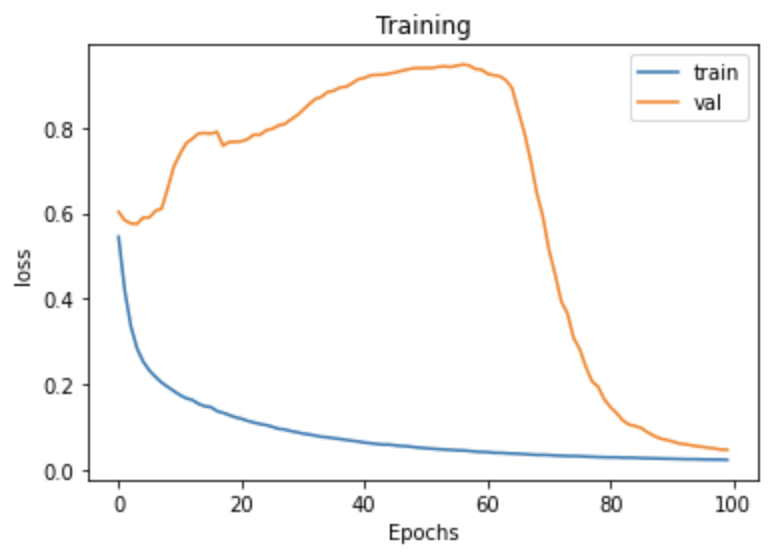
\includegraphics[width=0.6\linewidth]{Materials/unetLoss}
	\caption{Training and validation loss while training (measured as DICE loss).}
	\label{unetLoss}
\end{figure}
The validation loss starts off by growing quite a lot before at around 65 epochs to drop very rapidly. This indicates that the model around this point finds one or more features in the images which are good to use for segmentation and turns the emphasis / weights for these features up quite quickly. The training loss seems to behave quite normally by dropping quite steadily.\\
For the \textbf{test set} we can report an average \textbf{f1 score} of \textbf{0.955}. This is quite high, and shows the model both generalizes and performs quite well.\\
In \autoref{unetPred} we see an example of an prediction along the ground truth for that prediction. The DICE coefficient for this prediction is 0.988. As we can see, and the DICE coefficient indicates, the prediction is quite good, with only some of the edges being a little imprecise.
 
\begin{figure}
	\centering
	\begin{subfigure}{0.35\linewidth}
		\centering
		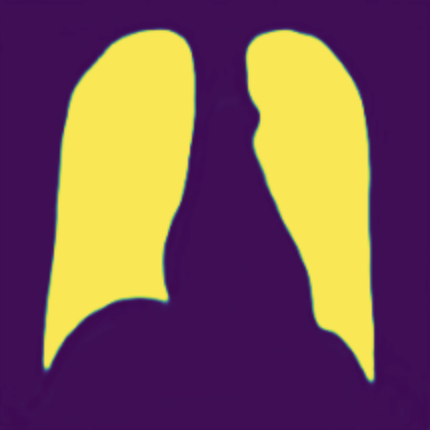
\includegraphics[width=\linewidth]{Materials/unetPred}
		\caption{Prediction.}
	\end{subfigure}
	\hspace{1cm}
	\begin{subfigure}{0.35\linewidth}
		\centering
		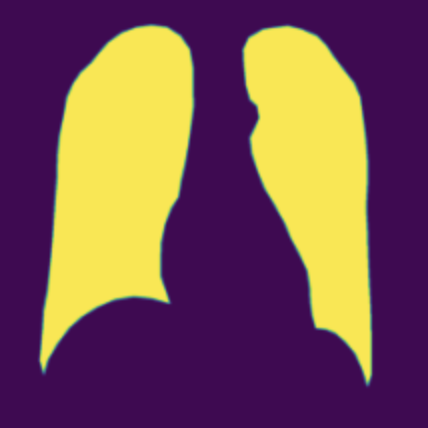
\includegraphics[width=\linewidth]{Materials/unetTrue}
		\caption{Ground truth.}
	\end{subfigure}	
	\caption{Model prediction and ground truth. Their DICE coefficient is 0.988.}
	\label{unetPred}
\end{figure}
%However, the model is not perfect, and although it scores high on average, it is not completely confident on all predictions as seen in \autoref{unConf}.
%
%\begin{figure}[h]
%	\centering
%	\begin{subfigure}{0.25\linewidth}
%		\centering
%		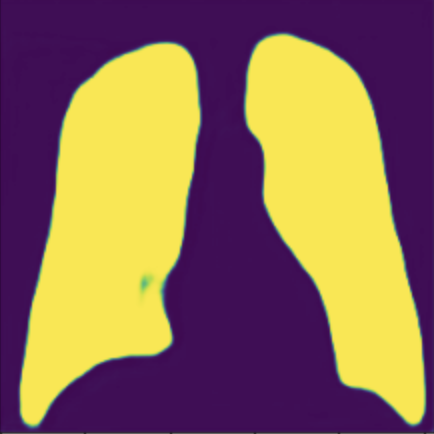
\includegraphics[width=\linewidth]{Materials/predUnconf}
%		\caption{Prediction.}
%	\end{subfigure}
%	\hspace{1cm}
%	\begin{subfigure}{0.25\linewidth}
%		\centering
%		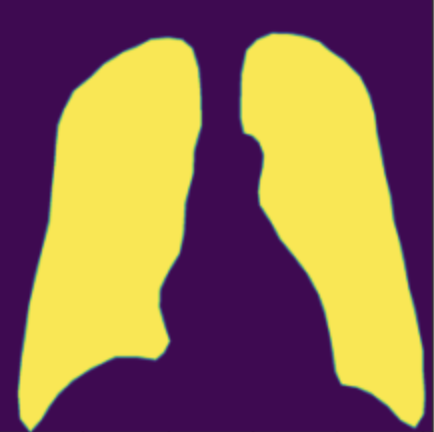
\includegraphics[width=\linewidth]{Materials/trueUnconf}
%		\caption{Ground truth.}
%	\end{subfigure}	
%	\caption{On this example, the model is not completely confident in its prediction.}
%	\label{unConf}
%\end{figure}